% \pdfminorversion=5
% \pdfcompresslevel=9
% \pdfobjcompresslevel=2
\documentclass[a4paper,12pt,reqno]{amsart}
\usepackage{M67tds}

% pour voir les solutions il faut enlever le commentaire de la ligne suivante
\solutionstrue

\newlist{axioms}{description}{1}
\newcommand\axiomlabel[1]{\hfill\textbf{(#1)}}
\setlist[axioms]{style=nextline,before={\let\makelabel\axiomlabel}}
\newcommand*{\ensemble}[3][]{#1\{ #2 \;#1|\; #3 #1\}} % par exemple \ensemble[\big]{x^2}{x \in \R}
\newcommand*{\abs}[1]{\left\lvert{\ifx\hfuzz#1\hfuzz \,\cdot\,\else#1\fi}\right\rvert} % la valeur absolue
\newcommand*{\axiom}[1]{\textbf{(#1)}}
\newcommand*{\overeq}[1]{\overset{\tiny{#1}}{=}}

% Les notes de bas de page dans les minipages (sidebyside)
\renewcommand{\thempfootnote}{\fnsymbol{mpfootnote}}

% pour surligner
\sisolutions{
  \usepackage{soul}
  \colorlet{hl}{yellow!35!white}
  \sethlcolor{hl}
}

\begin{document}

% ==================================
\hautdepage{

\ifsolutions{Solutions du devoir surveillé}\else{Devoir surveillé}\fi\par\normalfont\normalsize
21 mai 2019\\{[ durée: 3 heures ]}\par
}
% ==================================
\sisujet{
  % {\fontencoding{U}\fontfamily{futs}\selectfont\char 66\relax}
  \tikz[baseline=(e.base)]{\NoAutoSpacing\node(e){!};\draw[red,ultra thick,line join=round,yshift=-.15ex](90:1em)--(210:1em)--(330:1em)--cycle;}
  \textbf{Documents autorisés :}\textit{Une feuille A4 recto-verso écrite à la main.}

  \vspace{17mm}
  \tsvp
}


%-----------------------------------
\begin{exo} (Construction à la règle et au compas)

    \begin{enumerate}
      \item
      \sidebyside{.7}{
          Soient $O$ et $I$ deux points distincts du plan. Construire à la règle et au compas à partir de ces deux points les sommets $A_1=I, A_2, \ldots, A_8$ d'un octogone régulier inscrit dans le cercle de centre $O$ et de rayon $OI$ (c.-à-d. des points $A_1=I,A_2,\ldots,A_8$ deux à deux distincts situés sur le cercle de centre $O$ passant par $I$ tels que $A_1A_2=A_2A_3=\cdots=A_7A_8=A_8A_1$).
      }{
        \raisebox{-28mm}[0pt][0pt]{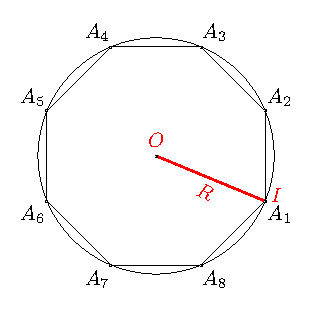
\includegraphics[width=4cm]{M67_2018-19_DS2_img_octogone}}
      }
      \item Déterminer l'aire de cet octogone régulier en fonction du rayon $R=OI$.
    \end{enumerate}
\end{exo}

\begin{solution}
    \begin{enumerate}
      \item
      \sidebyside{.7}{
        On pose $A_1=I$. Soit $A_5$ le second point d'intersection de $(OI)$ et du cercle $\mathcal{C}$ de centre $O$ passant par $I$. Les cercles de centre $A_1$ passant par $A_5$ et de centre $A_5$ passant par $A_1$ se coupent en deux points $J$ et $K$. La droite $(JK)$, médiatrice de $[A_1A_5]$, coupe le cercle $\mathcal{C}$ en deux points, $A_3$ et $A_5$. Le cercle de centre $A_1$ passant par $O$ et celui de centre $A_3$ passant par $O$ se recoupent en un point $L$. La droite $(OL)$, bissectrice de l'angle $\widehat{A_1OA_3}$ coupe le cercle en deux points, $A_2$, sur la demi-droite $[OL)$, et $A_6$. Le cercle de centre $A_3$ passant par $A_2$ recoupe $\mathcal{C}$ en $A_4$, et le cercle de centre $A_7$ passant par $A_6$ recoupe $\mathcal{C}$ en $A_8$.
      }{
        \raisebox{-49mm}[0pt][0pt]{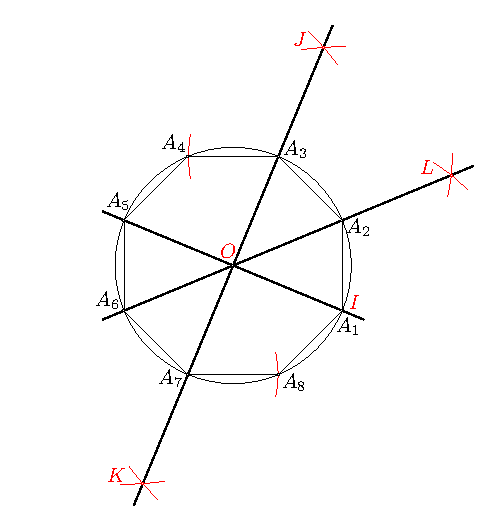
\includegraphics[width=4.9cm]{M67_2018-19_DS2_img_construction_octogone}}
      }
      \item Les huit triangles $\tri A_1OA_2$, $\tri A_2OA_3$, \dots, $\tri A_7OA_8$ et $\tri A_8OA_1$ étant égaux, ils ont même aire, et l'aire $\mathcal{A}$ de l'octogone est donc égale à $8 \cdot \mathcal{A}_{\tri A_1OA_2}$. D'autre part, l'angle $\widehat{A_1OA_2}$ vaut $\displaystyle{\frac{1}{8} \cdot 2\pi = \frac{\pi}{4}}$. Ainsi, l'aire du triangle $\tri A_1OA_2$ vaut $\displaystyle{OA_1 \cdot OA_2 \cdot \sin \frac{\pi}{4}=R^2\frac{\sqrt{2}}{2}}$. L'aire de l'octogone est donc égale à:
      \[
        \mathcal{A}=4\sqrt{2} R^2.
      \]
    \end{enumerate}
\end{solution}


%-----------------------------------
\begin{exo} (Quadrilatère «des milieux»)

  Étant donné un quadrilatère convexe (dit \emph{«de départ»}) on appelle \emph{«quadrilatère des milieux»} le quadrilatère convexe dont les sommets sont les milieux des côtés du quadrilatère de départ.
  \begin{enumerate}
    \item Montrer que quel que soit le quadrilatère de départ, le quadrilatère des milieux est un parallélogramme.
    \item Quel est le rapport entre l'aire du quadrilatère de départ et l'aire du quadrilatère des milieux ?
    \item Si le quadrilatère de départ est lui-même un parallélogramme, sous quelle condition le quadrilatère des milieux est-il un rectangle? et un carré?
  \end{enumerate}
\end{exo}

\begin{solution}

  \begin{enumerate}
    \item Soient $ABCD$ un quadrilatère convexe (ou non: la convexité n'est pas nécessaire pour cette première question), et $I$ le milieu de $[AB]$, $J$ celui de $[BC]$, $K$ celui de $[CD]$ et $L$ celui de $[DA]$. La droite $(IJ)$ passe par les milieux des côtés $[AB]$ et $[BC]$ du triangle $\tri ABC$, et est donc parallèle à $(AC)$. La droite $(KL)$ passe par les milieux des côtés $[CD]$ et $[DA]$ du triangle $\tri ACD$, et est donc parallèle à $(AC)$. Les droites $(IJ)$ et $(KL)$ étant toutes deux parallèles à $(AC)$ sont parallèles entre elles. On montre de même que $(IL)$ et $(JK)$ sont parallèles entre elles, car toutes deux parallèles à $(BD)$. Le quadrilatère $IJKL$ est donc un parallélogramme.
    \begin{center}
      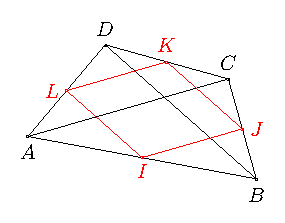
\includegraphics[width=4.9cm]{M67_2018-19_DS2_img_quadrilatere_milieux}
    \end{center}
    \item On conserve les notations de la première question. Comme le triangle $\tri AIL$ est homothétique de rapport $\frac{1}{2}$ à $\tri ABD$ nous avons la relation des aires $\mathcal{A}_{\tri AIL} = \frac{1}{4} \mathcal{A}_{\tri ABD}$. Et de même pour les trois autres triangles complémentaires au parallélogramme $IJKL$. Donc on trouve
    \begin{align*}
      \mathcal{A}_{ABCD} - \mathcal{A}_{IJKL}
        & = \mathcal{A}_{\tri AIL} + \mathcal{A}_{\tri BJI} + \mathcal{A}_{\tri CJK} + \mathcal{A}_{\tri DKL} \\
        & = \frac{1}{4}\left( \mathcal{A}_{\tri ABD} + \mathcal{A}_{\tri BCA} + \mathcal{A}_{\tri CDB} + \mathcal{A}_{\tri DAC} \right)\\
        &  = \frac{1}{4}.2.\mathcal{A}_{ABCD} = \frac{1}{2}\mathcal{A}_{ABCD}.
    \end{align*}
    Ainsi au final le rapport des aires est $\mathcal{A}_{IJKL}:\mathcal{A}_{ABCD} = \frac{1}{2}$.
    \item Nous avons les équivalences «le parallélogramme $IJKL$ est un rectangle» $\Leftrightarrow$ $(IJ) \perp (JK)$ $\Leftrightarrow$ $(AC) \perp (BD)$ $\Leftrightarrow$ «le parallélogramme $ABCD$ est un losange».\\
    De plus, en utilisant que $IJ=\frac{1}{2}AC$ et $KL=\frac{1}{2}BD$, nous avons $IJ=KL$ $\Leftrightarrow$ $AC=BD$. Ainsi «le parallélogramme $IJKL$ est un carré» $\Leftrightarrow$ «le parallélogramme $ABCD$ est un losange à diagonales égales» $\Leftrightarrow$ «le parallélogramme $ABCD$ est un carré».
  \end{enumerate}
\end{solution}


%-----------------------------------
\begin{exo} (Triangle rectangle et cercles)

  \begin{enumerate}
    \item Soit $ABC$ un triangle rectangle en $C$. Soient $a=BC$ et $b=AC$ les longueurs des côtés de l'angle droit. Montrer que la longueur $h$ de la hauteur issue de $C$ vérifie
    \[
      \frac{1}{h^2}=\frac{1}{a^2}+\frac{1}{b^2}.
    \]
    \item Soit $\mathcal{C}_1$ un cercle de diamètre $[OM]$. Soit $A$ un point de $\mathcal{C}_1$ différent de $O$ et $M$. Soit $\mathcal{C}_2$ le cercle de centre $O$ passant par $M$. On note $B$ et $C$ les points d'intersection de $(OA)$ et $\mathcal{C}_2$. Montrer que
    \[
      \frac{1}{MB^2} +\frac{1}{MC^2} = \frac{1}{MA^2}.
    \]
    \item Exprimer les longueurs des arcs $\wideparen{MB}$ et $\wideparen{MC}$ de $\mathcal{C}_2$ en fonction des longueurs des arcs $\wideparen{AO}$ et $\wideparen{AM}$ de $\mathcal{C}_1$.\footnote{On considère toujours l'arc le plus court: par exemple dans le cas de $\wideparen{MB}$ on parle de l'arc ne contenant pas $C$, dans le cas de $\wideparen{AM}$ on parle de l'arc ne contenant pas $O$.}
  \end{enumerate}
\end{exo}

\begin{solution}
  \begin{enumerate}
    \item L'aire du triangle rectangle $\tri ABC$ s'exprime comme $\frac{1}{2} \cdot BC \cdot AC = \frac{ab}{2}$ ou comme $\frac{1}{2} \cdot AB \cdot h$, d'où, en notant $c=AB$, $ab=ch$. D'après Pythagore, $c^2=a^2+b^2$, et donc $ \frac{1}{h^2}= \frac{c^2}{(ab)^2} =\frac{1}{a^2}+\frac{1}{b^2}$.
    \item Considérons le triangle $\tri BCM$. Comme $[BC]$ est un diamètre de $\mathcal{C}_2$ et $M \in \mathcal{C}_2$, ce triangle est rectangle en $M$. D'autre part, $A$,$M$ et $O$ sont sur $\mathcal{C}_1$ dont $[OM]$ est un diamètre. Le triangle $\tri MAO$ est donc rectangle en $A$, ce qui signifie que $[AH]$ est la hauteur de $BCM$ issue de $A$. L'égalité résulte alors de la question précédente.
    \begin{center}
      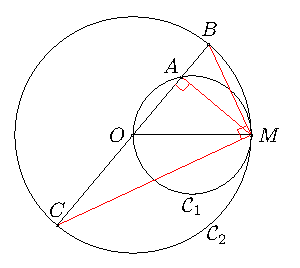
\includegraphics[width=4.9cm]{M67_2018-19_DS2_img_triangle_rectangle_cercles}
    \end{center}
    \item Supposons pour fixer les notations que $B$ soit le point d'intersection de $[OA)$ et de $\mathcal{C}_2$. Notons $R_1=\frac{OM}{2}$ et $R_2=OM$ les rayons de $\mathcal{C}_1$ et $\mathcal{C}_2$. La longueur de l'arc $\wideparen{BM}$ est égale à $R_2 \cdot \widehat{BOM}$ (où $\widehat{BOM}$ est exprimée en radians). Mais $\widehat{BOM}=\widehat{AOM}$ est dans $\mathcal{C}_1$ un angle inscrit qui intercepte l'arc $\wideparen{AM}$. L'arc $\wideparen{AM}$ mesure donc $R_1 \cdot \frac{1}{2}\widehat{AOM}$. Autrement dit, les arcs $\wideparen{AM}$ et $\wideparen{BM}$ ont la même longueur.\\
    Les points $B$ et $C$ sont diamétralement opposés. Ainsi la somme des arcs $\wideparen{MB}$ et $\wideparen{MC}$ est égale au demi-périmètre du cercle $\mathcal{C}_2$, soit le double de la longueur de l'arc $\wideparen{OM}$ de $\mathcal{C}_1$. La longueur $l(\wideparen{CM})$ de l'arc $\wideparen{CM}$ vaut donc $l(\wideparen{CM})=l(\wideparen{BC})-l(\wideparen{BM})=2(l(\wideparen{OA})+l(\wideparen{AM}))-l(\wideparen{AM})=2l(\wideparen{OA})+l(\wideparen{AM})$.
  \end{enumerate}
\end{solution}



%-----------------------------------
\begin{exo}[.7] (Kangourou 2019)

  \sidebyside{.7}{
    La figure ci-contre est faite de trois cercles de même rayon $R$ dont les centres sont alignés. Le cercle du milieu passe par les centres des deux autres. Quel est le périmètre de cette figure?
  }{
    \raisebox{-14mm}[0pt][0pt]{\includegraphics[width=4cm]{img_kangourou2019j}}
  }
\end{exo}

\begin{solution}
  \sidebyside{.7}{
    Les triangles rouges sur la figure ci-contre sont équilatéraux, donc le périmètre est constitué de deux arcs de \textcolor{blue}{$240°$} et de deux arcs de \textcolor{purple}{$60°$}. Ainsi le périmètre est de $2 \frac{4\pi}{3}R + 2 \frac{\pi}{3}R = \frac{10}{3}\pi R$.
  }{
    \raisebox{-14mm}[0pt][0pt]{\includegraphics[width=4cm]{img_kangourou2019js}}
  }
\end{solution}



\end{document}
